% ----------------------------------------------------------------------
%  Před psaním se důkladně seznamte s Pravidly pro vypracování protokolu!
% ----------------------------------------------------------------------

% ----------------------------------------------------------------------
%  Pracovní úkoly - opište přímo ze zadání
% ----------------------------------------------------------------------
\section{Pracovní úkoly}

\begin{enumerate}
\item ...

\end{enumerate}

% ----------------------------------------------------------------------
%  Použité pomůcky
% ----------------------------------------------------------------------

\newpage


%\begin{figure}[H]
%	\centering
%	\includegraphics[scale = 0.5]{img/schema_regulovane_soustavy.png} 
%	\caption{Schéma regulované soustavy.} 
%	\label{fig:schema_reg}
%\end{figure}	

%\begin{figure}[H] 
%	\centering
%	\includegraphics[scale = 0.7]{img/schema_PID_regulatoru.png} 
%	\caption{Schéma PID regulátoru.} 
%	\label{fig:schema_PID}
%\end{figure}		
		

% ----------------------------------------------------------------------
%  Teoretický úvod - vlastními slovy stručne popište fyzikální podstatu měření a uveďte základní vztahy použité ve vypracování
% ----------------------------------------------------------------------
%\section{Teoretický úvod}	

% ----------------------------------------------------------------------
%  Postup měření - vlastními slovy popište postup měření tak, aby bylo vaše měření reprodukovatelné 
% ----------------------------------------------------------------------
%\section{Postup měření}
			
% ----------------------------------------------------------------------
%  Naměřené hodnoty a samotné vypracování úkolu
% ----------------------------------------------------------------------	
			
\section{Vypracování}
\subsection{Charakteristika laseru v režimu volné generace}

\begin{table}[!hbt]
\centering
	\begin{tabular}{|c|c|c||c|c|c||c|c|c|}
		\hline
		\multicolumn{3}{|c||}{M337}					&	\multicolumn{3}{c||}{křemenné sklo}					&	\multicolumn{3}{c|}{M327}					\\ \hline
$\tabh{E_\mathrm{b}}{J}$	&	\tabh{E}{J}	&	\tabh{\eta}{\%}	&	$\tabh{E_\mathrm{b}}{J}$	&	\tabh{E}{J}	&	\tabh{\eta}{\%}	&	$\tabh{E_\mathrm{b}}{J}$	&	\tabh{E}{J}	&	\tabh{\eta}{\%}	\\ \hline \hline
13,62	&	0,00	&	0,00	&	15,21	&	0,00	&	0,00	&	13,76	&	0,00	&	0,00	\\ \hline
14,14	&	0,02	&	0,16	&	16,89	&	0,02	&	0,11	&	14,14	&	0,02	&	0,15	\\ \hline
15,21	&	0,04	&	0,29	&	19,27	&	0,08	&	0,40	&	15,21	&	0,07	&	0,45	\\ \hline
16,89	&	0,07	&	0,39	&	22,37	&	0,15	&	0,68	&	16,89	&	0,13	&	0,74	\\ \hline
19,27	&	0,10	&	0,50	&	26,52	&	0,24	&	0,89	&	19,27	&	0,19	&	1,01	\\ \hline
22,37	&	0,14	&	0,60	&	31,70	&	0,35	&	1,10	&	22,37	&	0,27	&	1,21	\\ \hline
26,52	&	0,19	&	0,71	&	34,22	&	0,39	&	1,14	&	26,52	&	0,34	&	1,30	\\ \hline
31,70	&	0,25	&	0,78	&	38,32	&	0,47	&	1,24	&	31,70	&	0,45	&	1,41	\\ \hline
38,32	&	0,33	&	0,87	&	42,90	&	0,56	&	1,30	&	38,32	&	0,58	&	1,51	\\ \hline
46,38	&	0,40	&	0,85	&	48,16	&	0,66	&	1,37	&	46,38	&	0,72	&	1,55	\\ \hline
56,25	&	0,51	&	0,90	&	56,25	&	0,81	&	1,44	&	56,25	&	0,89	&	1,58	\\ \hline

	\end{tabular}
	\caption{Závislosti výstupní energie $E$ a účinnosti $\eta$ na budící energii $E_\mathrm{b}$ pro zrcadla M337, M327 a křemenné sklo.}
	\label{tab:ucinnost_zrcadla}
\end{table}

\begin{figure}[H] 
	\centering
	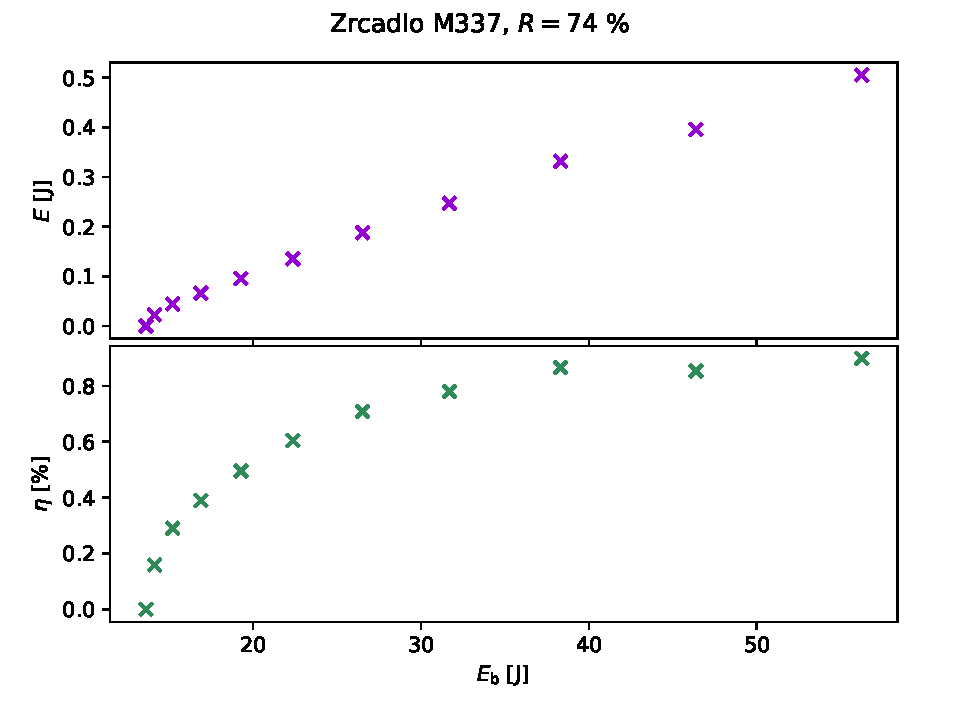
\includegraphics[scale = 0.7]{img/zrcadlo_M337.pdf} 
	\caption{Závislost výstupní energie $E$ a účinnosti $\eta$ na budící energii $E_\mathrm{b}$ pro zrcadlo M337.} 
	\label{fig:ucinnost_M337}
\end{figure}


\begin{figure}[H] 
	\centering
	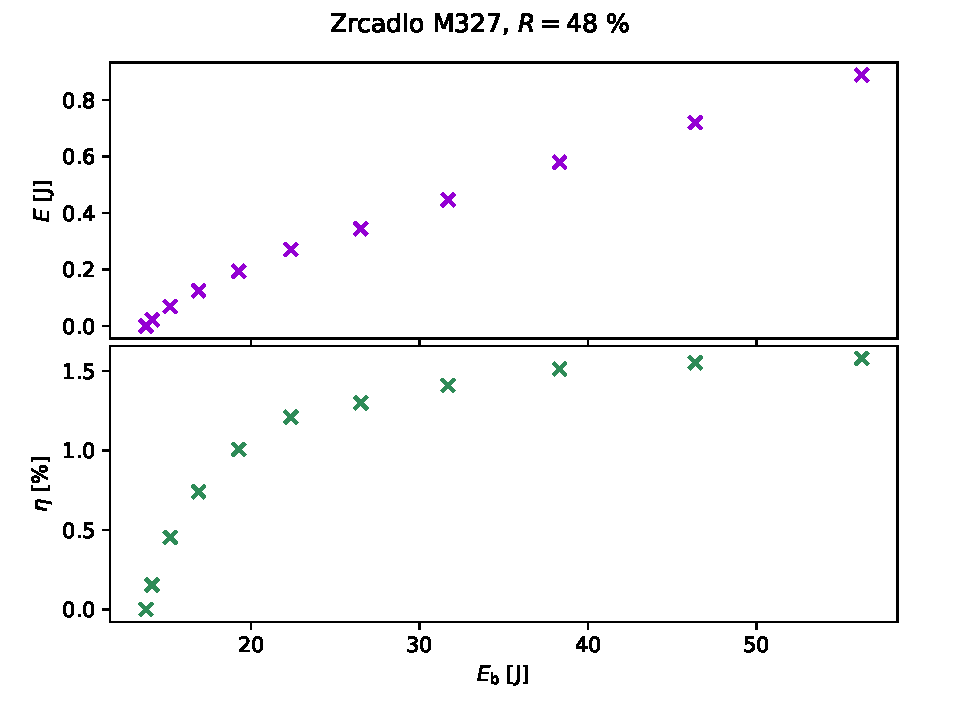
\includegraphics[scale = 0.7]{img/zrcadlo_M327.pdf} 
	\caption{Závislost výstupní energie $E$ a účinnosti $\eta$ na budící energii $E_\mathrm{b}$ pro zrcadlo M327.} 
	\label{fig:ucinnost_M327}
\end{figure}


\begin{figure}[H] 
	\centering
	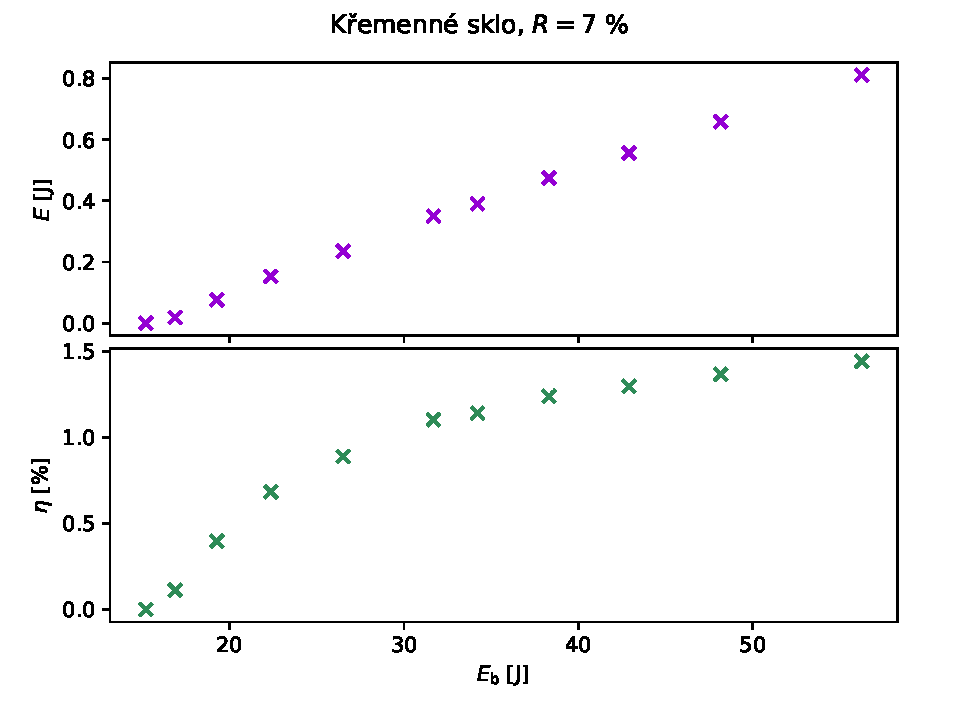
\includegraphics[scale = 0.7]{img/zrcadlo_kremenne_sklo.pdf} 
	\caption{Závislost výstupní energie $E$ a účinnosti $\eta$ na budící energii $E_\mathrm{b}$ pro zrcadlo z křemenného skla.} 
	\label{fig:ucinnost_kremenne_sklo}
\end{figure}

\begin{figure}[H] 
	\centering
	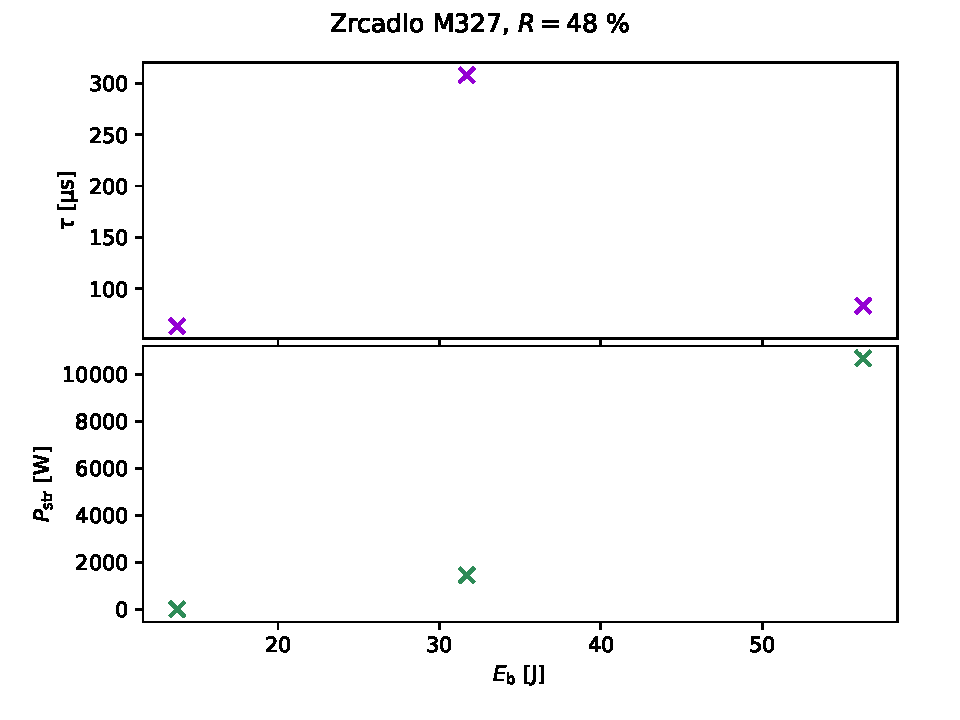
\includegraphics[scale = 0.7]{img/optimalni_zrcadlo.pdf} 
	\caption{Závislost délky impulsu $\tau_\mathrm{FR}$, a středního výkonu $P_\mathrm{str}$ na budící energii $E_\mathrm{b}$ pro zrcadlo M327.} 
	\label{fig:ucinnost_kremenne_sklo}
\end{figure}
% ----------------------------------------------------------------------
%  Diskuse - obsahuje komentář k jednotlivým výsledkům, porovnání s očekáváním/tabulkovými hodnotami, zdroje především systematických chyb měření, návrh na zlepšení výsledků,...
% ----------------------------------------------------------------------			
%\section{Diskuse}			

% ----------------------------------------------------------------------
%  Závěr - stručně a jasně shrnout splněné cíle měření, úkoly a výsledky měření
% ----------------------------------------------------------------------
			
%\section{Závěr}



